\documentclass[xcolor=dvipsnames,aspectratio=169]{beamer}

% INCLUSIÓN DOS PAQUETES IMPRESCINDIBLES DE IDIOMA E CODIFICACIÓN DE CARACTERE.
\usepackage[T1]{fontenc}
\usepackage[english]{babel}
\usepackage[utf8]{inputenc}
\usepackage{csquotes}

%ACRONYMS para engadir un glosario de acronimos automatizado
% \usepackage[acronyms,nonumberlist,nopostdot,nomain,nogroupskip]{glossaries}
% \input{./acronyms.tex}

% PAQUETES PARA FIGURAS E GRAFICOS
\usepackage{graphicx}
%   \usepackage[pdftex]{graphicx}
  \usepackage{epstopdf}
   \graphicspath{{./img/}}
  % and their extensions so you won't have to specify these with
  % every instance of \includegraphics
   \DeclareGraphicsExtensions{.eps,.pdf,.png,.jpg}   
\usepackage{subfigure}
\usepackage{caption}

%Tikz plots
\usepackage{tikz}
\usepackage{tikzscale}
\usetikzlibrary{plotmarks,patterns,decorations.pathreplacing,backgrounds,calc,arrows,arrows.meta,spy,matrix,backgrounds,shapes}

\tikzset{
    block/.style = {draw, rectangle, 
        minimum height=1cm, 
        minimum width=1.2cm},
    input/.style = {coordinate,node distance=1cm},
    output/.style = {coordinate,node distance=2cm},
    arrow/.style={draw, -latex,node distance=1.5cm},
    pinstyle/.style = {pin edge={latex-, black,node distance=1.5cm}},
    sum/.style = {draw, circle, node distance=1cm}
}
\newcommand{\tikzmark}[1]{\tikz[overlay,remember picture] \UE (#1) {};}
\newcommand{\DrawBox}[4][]{%
    \tikz[overlay,remember picture]{%
        \coordinate (TopLeft)     at ($(#2)+(-0.4em,1.6em)$);
        \coordinate (BottomRight) at ($(#3)+(0.4em,-1.0em)$);
        %
        \path (TopLeft); \pgfgetlastxy{\XCoord}{\IgnoreCoord};
        \path (BottomRight); \pgfgetlastxy{\IgnoreCoord}{\YCoord};
        \coordinate (LabelPoint) at ($(\XCoord,\YCoord)!0.5!(BottomRight)$);
        %
        \draw [red,#1] (TopLeft) rectangle (BottomRight);
        \UE [below, #1, fill=none, fill opacity=1] at (LabelPoint) {#4};
    }
}
\usepackage{pgfplots}
\pgfplotsset{compat=newest}
\pgfplotsset{plot coordinates/math parser=false}
\usepgfplotslibrary{patchplots,groupplots}

% OUTROS PAQUETES DE USO COMUN. HOXE EN DIA OS COMPILADORES SON TAN RAPIDOS QUE EU METO TODOS SEMPRE
% \usepackage{float}
% \usepackage{ucs} 
% \usepackage{subcaption}
\usepackage{psfrag}
\usepackage{verbatim}
\usepackage{amsmath}
\usepackage{amsfonts} 
\usepackage{amssymb} 
\usepackage{amsthm}
\usepackage{pifont}
\usepackage{array}
\usepackage{listings}
\usepackage{stfloats}
\usepackage{algorithm} 
\usepackage{algorithmic} 
\usepackage{url} 
\usepackage{enumerate}
\usepackage{multirow}
\usepackage{wasysym}
\usepackage{cancel}
\usepackage{lmodern}
\usepackage{mathrsfs}

\input{EETbeamerconfig.tex}
\input{mydefinitions.tex}

%---------------
% LIMIAR
%---------------
%configuracion de opcions de beamer persoais, pero alleas ao estilo

% COMANDO QUE INTRODUCE UNHA DIAPOSITIVA CUN ÍNDICE NO QUE APARECEN VELADAS TÓDALAS SECCIÓNS MENOS A ACTUAL. ÚTIL PARA INTRODUCIR OS TÍPICOS ÍNDICES INTERMEDIOS.
\newcommand{\Inter}{\frame{\tableofcontents[currentsection]}}
\newcommand{\inter}{\frame{\tableofcontents[currentsection,currentsubsection]}}

% Pes de imaxe
\renewcommand{\figurename}{Fig.}
\addto\captionsenglish{\renewcommand{\figurename}{Fig.}}
\setbeamertemplate{caption}[numbered]

%ESTE PAQUETE PERMITE POÑER A BIBLIOGRAFIA AO PE DE PAXINA CON CONFIGURACIONS ESTETICAS PERSOAIS
% \usepackage[style=ieee,doi=false,isbn=false,url=true,backend=bibtex]{biblatex}
% \bibliography{./bibliografia.bib}
% \newrobustcmd*{\footfullcitenomark}{%
%   \AtNextCite{%
%     \let\thefootnote\relax 
%     \let\mkbibfootnote\mkbibfootnotetext
%     }%
%   \footfullcite}

%paquete para engadir notas de guion ao pdf
\usepackage{pgfpages}
% \setbeameroption{show only notes} 
% \setbeameroption{show notes}
% \setbeameroption{show notes on second screen=right}
% DATOS DO DOCUMENTO
\title{Advanced Communication Systems}
\subtitle{Part 2.2:\\ Multi-user Communications:\\ Broadcast Channel}
\author[FGC]{Felipe G\'omez Cuba}
\institute[XX]{
\begin{columns}[T]
\begin{column}{9cm}\centering
Despacho 204\\
Titorías: Lun-Xov 15:00-16:30\\
(En caso de confinamento: videochamada a calquera horario acordado)\\
  \texttt{gomezcuba@gts.uvigo.es}\\
\end{column}
\end{columns}
}

\date{2 \& 4 \& 9 November 2020 }

\begin{document}

% Diapositiva co título
%\frame[plain]{\titlepage}%the ``classic'' beamer cover pageç

\frame{\frametitle{\\}%generate top bar, but blank line as tittle
\titlepage
}%approximation to the ``GPSC ppt'' cover page, but with central beamer title

% \frame{\tableofcontents}
% \note[itemize]{%itemized notes are special ``note'' slides that beamer can append to the pdf or not, depending on a boolean toggle option
% \item Introduce yourself
% \item In this work we studied blablabla.
% }

% \section{IAB MmWave Network}

\frame[allowframebreaks]{\frametitle{Broadcast Channel}
        \begin{figure}
            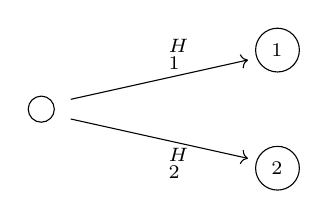
\begin{tikzpicture}[scale=.5]
                \draw [->] (.75,0.25) -- (5.25,1.25);
                \draw [->] (.75,-0.25) -- (5.25,-1.25);
                \node[draw,circle] at (6,1.5) {$\y_1$};
                \node[draw,circle] at (6,-1.5) {$\y_2$};
                \node[draw,circle] at (0,0) {$\x$};
                \node[anchor=south] at (3.5,.75) {$\Hb_1^H$};
                \node[anchor=north] at (3.5,-.75) {$\Hb_2^H$};
            \end{tikzpicture}
            \end{figure}


    \begin{itemize}
     \item Directed graph with one transmitter and $K$ receivers
     \begin{itemize}
        \item Each user $k$ decodes signal $\y_k$ \textit{independently}
        \item General case $(Y_1,\dots Y_K) \sim f((\y_1\dots \y_K)|\x)$ (dependent)\\ \ \\
    \end{itemize}
    \item AWGN BC channel
        $$\y_k = \Hb_k^H\x+\z_k\; \forall k\in\{1\dots K\}$$ 
     \item Channel Reciprocity: $\Hb_k$ in MAC $\to$ $\Hb_k^H$ in BC\\ \ \\
     \item Example: \textit{Downlink} in a mobile cellular system\\ \ \\
     \item All devices may have one or multiple antennas\\ \ \\
     \item Independent message to each $k$ with rate $R_k$
     \begin{itemize}
        \item Do not confuse with the expression ``TV Broadcast''\\ \ \\
    \end{itemize}
     \item \textit{One possible way} to generate $\x$ is
        $$\x=\sum_{k=1}^{K}\x_k\to \y_k = \Hb_k^H\left(\sum_{k'=1}^{K}\x_{k'}\right)+\z_k$$
     \item Difference with MAC: same $\Hb_k^H$ multiplies all $\x_{k'}$'s
    \end{itemize}
}

\frame{\frametitle{2-user AWGN SISO BC Capacity Region}
    \begin{itemize}
     \item Assume $K=2$, $N_{t}=N_{r1}=N_{r2}=1$, and $|h_1|<|h_2|$
     \item<3-> $|h_1|<|h_2|\to$ ``U2 can decode everything U1 can decode''
    \end{itemize}
        \begin{equation}
        \mathcal{C}\subset \left\{
            \begin{array}{rl}
                \onslide<1->{
                    \textcolor{ARust}{R_1}&\textcolor{ARust}{\leq \log(1+\frac{P|h_1|^2}{BN_o})}\\
                    }
                \onslide<2->{
                    \textcolor{VCobalt}{R_2}&\textcolor{VCobalt}{\leq \log(1+\frac{P|h_2|^2}{BN_o})}\\
                    }
                \onslide<3->{
                    \textcolor{KYJade}{ R_1+R_2}&\textcolor{KYJade}{ \leq \log(1+\frac{P_1|h_1|^2+P_2|h_2|^2}{BN_o})}
                    }
            \end{array}
        \right\}
        \end{equation}
        
%         \onslide<3->{$$\textnormal{ choosing } \x=\sqrt{\frac{P_1}{P}}\x_1+\sqrt{\frac{P_2}{P}}\x_2$$}

    \begin{columns}
        \begin{column}{6cm}
        \begin{figure}
            \begin{tikzpicture}[scale=.5]
                \draw [->] (.75,0.25) -- (5.25,1.25);
                \draw [->] (.75,-0.25) -- (5.25,-1.25);
                \node[draw,circle] at (6,1.5) {$y_1$};
                \node[draw,circle] at (6,-1.5) {$y_2$};
                \node[draw,circle] at (0,0) {$x$};
                \node[anchor=south] at (3.5,.75) {$h_1^*$};
                \node[anchor=north] at (3.5,-.75) {$h_2^*$};
                 \onslide<1->{
                 \draw [ARust,dashed,domain=-90:45] plot ({6-1.3*cos(\x)}, {1.5+1.3*sin(\x)});
                 \node[color=ARust,anchor=south] at (5,2.5) {$x=x_1$};
                 }
                 \onslide<2->{
                 \draw [VCobalt,dashed,domain=-45:90] plot ({6-1.3*cos(\x)}, {-1.5+1.3*sin(\x)});
                 \node[color=VCobalt,anchor=north] at (5,-2.5) {$x=x_2$};
                 }
                 \onslide<3->{
                    \draw [KYJade,dashed,domain=-45:45] plot ({6-2*cos(\x)}, {4*sin(\x)});
                    \node[color=KYJade,anchor=east] at (4,2.25) {$x=\sqrt{\frac{P_1}{P}}x_1+\sqrt{\frac{P_2}{P}}x_2$};
                    }
            \end{tikzpicture}
            \end{figure}
        \end{column}
        \begin{column}{6cm}
            \begin{figure}
            \begin{tikzpicture}[scale=.9]
                \draw[help lines,color=gray,dotted] (0,0) grid (4,4);
%          \onslide<3->{\fill[color=yellow!25] (0,0) -- (3,0) -- (3,1) -- (1,3) -- (0,3) -- (0,0);}      
                \draw [->] (0,0) -- (0,4.2);
                \draw [->] (0,0) -- (4.2,0);
                \node [anchor=north] at (2,-0.3) {$R_1$}; 
                \node [anchor=east] at (-0.3,4) {$R_2$}; 
% %                 \foreach \x in {0,1,...,4} { \node [anchor=north] at (\x,-0.3) {\tiny \x}; }
% %                 \foreach \y in {0,1,...,4} { \node [anchor=east] at (-0.3,\y) {\tiny \y}; }          
         \onslide<1->{\draw[color=ARust,thick] (3,-.5) -- (3,.5);}                
         \onslide<2->{\draw[color=VCobalt,thick] (-.5,4) -- (.5,4);}
%          
%          \onslide<3->{
%             \draw[color=gray,dotted] (0,0) -- (2,2);  
         \onslide<3->{         
% %             \note [name=p1] at (ln(1+7.1*.25/1.75)/ln(2), ln(1+15*.75)/ln(2)) {};
% %             \note [name=p2] at  (ln(1+7.1*.25)/ln(2), ln(1+15*.75/1.25)/ln(2)) {};
            \coordinate (A) at ({ln(1+7.1*.25)/ln(2)}, {ln(1+15*.75/1.25)/ln(2)});
            \coordinate (B) at ({ln(1+7.1*.25/1.75)/ln(2)}, {ln(1+15*.75)/ln(2)});
            \draw[KYJade] (B) circle (.1);
            \fill[KYJade] (B) circle (.1);
            }
         \onslide<3-3>{ 
            \draw[KYJade,dashed] (A |- 0,0) -- (A) -- (B) -- (0,0 |- B);
            \node[color=KYJade,anchor=west] at (B) {$P_2=\frac{3}{4}P$};
         }
         \onslide<4->{         
% %             \note [name=p1] at (ln(1+7.1*.25/1.75)/ln(2), ln(1+15*.75)/ln(2)) {};
% %             \note [name=p2] at  (ln(1+7.1*.25)/ln(2), ln(1+15*.75/1.25)/ln(2)) {};
            \coordinate (A) at ({ln(1+7.1*.5)/ln(2)}, {ln(1+15*.5/1.5)/ln(2)});
            \coordinate (B) at ({ln(1+7.1*.5/1.5)/ln(2)}, {ln(1+15*.5)/ln(2)});
            \draw[KYJade] (B) circle (.1);
            \fill[KYJade] (B) circle (.1);
            }
         \onslide<4-4>{ 
            \draw[KYJade,dashed] (A |- 0,0) -- (A) -- (B) -- (0,0 |- B);
            \node[color=KYJade,anchor=west] at (B) {$P_2=\frac{1}{2}P$};
         }
         \onslide<5->{         
% %             \note [name=p1] at (ln(1+7.1*.25/1.75)/ln(2), ln(1+15*.75)/ln(2)) {};
% %             \note [name=p2] at  (ln(1+7.1*.25)/ln(2), ln(1+15*.75/1.25)/ln(2)) {};
            \coordinate (A) at ({ln(1+7.1*.8)/ln(2)}, {ln(1+15*.2/1.8)/ln(2)});
            \coordinate (B) at ({ln(1+7.1*.8/1.2)/ln(2)}, {ln(1+15*.2)/ln(2)});
            \draw[KYJade,dashed] (A |- 0,0) -- (A) -- (B) -- (0,0 |- B);
            \draw[KYJade] (B) circle (.1);
            \fill[KYJade] (B) circle (.1);
            }
         \onslide<5-5>{ 
            \node[color=KYJade,anchor=west] at (B) {$P_2=\frac{1}{5}P$};
            \draw[KYJade,dashed] (A |- 0,0) -- (A) -- (B) -- (0,0 |- B);
         }
         \onslide<6->{         
            \draw [KYJade,domain=1:99] plot ({ln(1+7.1*\x/100/(2-\x/100))/ln(2)}, {ln(1+15*(100-\x)/100)/ln(2)});
            }
% %          \onslide<3->{\node at (1,1) {$\mathcal{C}$}; }
         
            \end{tikzpicture}
            \end{figure}
        \end{column}
    \end{columns}
}

\frame{\frametitle{Degraded BC Channel}
\begin{definition}
 A general 2-user BC channel is said to be \textbf{degraded} if its p.d.f. can be written as $f(Y_1,Y_2|X)=f(Y_2|Y_1)f(Y_1|X)$.
\end{definition}
\begin{theorem}[Capacity of Degraded BC Channel $X\to Y_1\to Y_2$]
 If we define an auxiliary random variable $V$ with distribution $f(v)$
 $$\mathcal{C}= \left\{\vec{R}:\begin{array}{rl}
    R_1&\leq \Inf{V}{Y_1}\\
    R_2&\leq \CInf{X}{Y_2}{V}\\
 \end{array}\forall f(v): |\mathcal{V}|\leq \min(|\mathcal{X}|,|\mathcal{Y}_1|,|\mathcal{Y}_2|)  \right\}$$
\end{theorem}
\begin{remark}
 The AWGN SISO MAC capacity region is an example of Degraded BC Channel with $v=x_1$ and $f(y_2,y_1)= f_{x_2}(y_2-y_1)f(y_1)$.
\end{remark}
\begin{itemize}
 \item We need to \textbf{order} the users defining a chain. Since there is no trivial ordering of vectors, MIMO BC is more difficult.
\end{itemize}
}


\frame{\frametitle{$K$-User SISO MAC Channel}
\begin{itemize}
 \item Consider the $K$-User SISO MAC Channel
    $$y_k=h_k\left(\sum_{k'=1}^{K}x_{k'}\right) + z_k$$
 \item Assume users are labeled in increasing channel order
    $$|h_1|\leq|h_2|\leq\dots\leq|h_K|$$
\end{itemize}

\begin{theorem}
 For each user $k$ in a $K$-User SISO MAC Channel, user $k$ can achieve rate
 $$R_k=B\log\left(1+\frac{P_k|h_k|^2}{BN_o+|h_k|^2\sum_{k'=k+1}^{K}P_{k'}}\right)$$ 
\end{theorem}
}


\frame{\frametitle{Superposition Coding}
\begin{itemize}
 \item Let $x_1 \in \mathcal{C}_1$, $x_2 \in \mathcal{C}_2$, and $\sqrt{\alpha}x_1+\sqrt{1-\alpha}x_2\triangleq x \in \mathcal{C}$
 \begin{figure}
  \begin{tikzpicture}[scale=.4]
    \draw[help lines,color=gray,dotted] (-3.2,-3.2) grid (3.2,3.2);
    \draw [<->] (0,-3.5) -- (0,3.5);
    \draw [<->] (-3.5,0) -- (3.5,0);
    \node[anchor=north] at (3,0) {\Tiny $\Re\{\x\}$};
    \node[anchor=east] at (0,3) {\Tiny $\Im\{\x\}$};
    \node[draw,cross=2pt] at (2,2) {};
    \fill[VCobalt] (2.5,2.5) circle (.2);
    \fill[VCobalt] (1.5,1.5) circle (.2);
    \fill[VCobalt] (2.5,1.5) circle (.2);
    \fill[VCobalt] (1.5,2.5) circle (.2);
    \node[draw,cross=2pt] at (-2,2) {};
    \fill[VCobalt] (-2.5,2.5) circle (.2);
    \fill[VCobalt] (-1.5,1.5) circle (.2);
    \fill[VCobalt] (-2.5,1.5) circle (.2);
    \fill[VCobalt] (-1.5,2.5) circle (.2);
    \node[draw,cross=2pt] at (2,-2) {};
    \fill[VCobalt] (2.5,-2.5) circle (.2);
    \fill[VCobalt] (1.5,-1.5) circle (.2);
    \fill[VCobalt] (2.5,-1.5) circle (.2);
    \fill[VCobalt] (1.5,-2.5) circle (.2);
    \node[draw,cross=2pt] at (-2,-2) {};
    \fill[VCobalt] (-2.5,-2.5) circle (.2);
    \fill[VCobalt] (-1.5,-1.5) circle (.2);
    \fill[VCobalt] (-2.5,-1.5) circle (.2);
    \fill[VCobalt] (-1.5,-2.5) circle (.2);
  \end{tikzpicture}
  \caption{QPSK $x_1$ combined with QPSK $x_2$}
  \end{figure}
  \item User 1 decodes $\mathcal{C}_1$\\ \ \\
  \item User 2 with ML $$\arg\max_{x\in\mathcal{C}}\|y_2-h_2x\|^2$$
  \item User 2 with DF $$\arg\max_{x_2\in\mathcal{C}_2}\|y_2-h_2\hat{x}_1-h_2x_2\|^2\leftarrow  \hat{x}_1=\arg\max_{\x_1\in\mathcal{C}_1}\|y_2-h_2x_1\|^2$$
\end{itemize}
}

\frame{\frametitle{Homework: Common Message BC}
% \begin{homework}
    We can generalize the BC to include the ``TV broadcast'' with the same message to all users, and intermediate cases.
    
    Consider a 2-user SISO Gaussian BC with $|h_1|<|h_2|$ with \textbf{three messages} and a \textbf{3D} rate vector $(R_c,R_1,R_2)$ defined as follows
    $$y_k=h_k (x_c+x_1+x_2)+z_k\quad\forall k \in\{1,2\}$$
    \vspace{-.3in}
    \begin{itemize}
     \item $x_c$ is a \textbf{commmon message} that both U1 and U2 want to decode.
     \item $x_1$ is the normal \textbf{individual message} U1 wants to decode.
     \item $x_2$ is the normal \textbf{individual message} U2 wants to decode.
    \end{itemize}
    
    Write a set of constraints that characterizes the \textbf{3D} region of achievable rate triplets $(R_c,R_1,R_2)\in\mathcal{C}_{CM-BC}$. (Hint: U2 \textbf{can} decode both $x_c$ and $x_1$, the only difference between these two messages is that U2 also wants to keep $x_c$ for themself after using it to cancel interference)

% \end{homework}
}
 
\frame[allowframebreaks]{\frametitle{MAC -- BC duality (SISO)}
\begin{lemma}
 The capacity region of the MAC channel with powers $\vec{P}=\left(P_1,P_2,\dots P_K\right)$ is a subset of the capacity region of the dual BC with power constraint $\displaystyle P=\sum_{k=1}^{K} P_k$.
\end{lemma}    
 \begin{remark}
    The boundaries intersect at exactly one point if the channel gains of all users are different.
 \end{remark}
\begin{theorem}[Capacity Region of the BC Channel]
 $$\mathcal{C}_{BC}=\bigcup_{\vec{P}:\sum_{k=1}^{K} P_k=P}\mathcal{C}_{MAC}(\vec{P},\h)$$
\end{theorem}    

\begin{definition}[Dual MAC {[DMAC]}]
A special MAC \textbf{with $K$ transmitted symbols}, freedom to choose transmitter power $\vec{P}^{DMAC}=(P_1^{DMAC},\dots,P_K^{DMAC})$, and \textbf{global} power constraint $\sum_{k=1}^{K} P^{DMAC}_k=P$.
    $$y^{DMAC}=\sum_{k=1}^K h_k x_k^{DMAC}+z^{DMAC}=(h_1\dots h_K)\x^{DMAC}+z^{DMAC}$$
\end{definition}

\begin{theorem}
 $\mathcal{C}_{DMAC}=\mathcal{C}_{BC}$, but for a given set of rates $\vec{R}\in\mathcal{C}_{BC}$ the power allocations that achieve it are not necessarily the same in both systems $\vec{P}^{DMAC}(\vec{R})\neq\vec{P}(\vec{R})$. 
\end{theorem}

\pagebreak

\begin{remark}[Boundary of $\mathcal{C}_{DMAC}$ as a Convex Optimization]
    We can fully compute the boundary of $\mathcal{C}_{DMAC}$ as the following convex optimization
    $$\max_{\vec{R},\vec{P}^{DMAC}} \left(\mu_1,\dots,\mu_K\right)\left(\begin{array}{c}R_1\\\vdots\\R_K\end{array}\right)\textnormal{ s.t. }\begin{cases}\sum_{k=1}^{K} P_k^{DMAC}=P\\\sum_{k=1}^{K} \mu_k=1\\ \vec{R}\in\mathcal{C}_{MAC}(\vec{P},\h) \end{cases}$$
    This convex problem is more tractable than a direct calculation of the boundary of $\mathcal{C}_{BC}$ (non-convex)
\end{remark}
\pagebreak

 \begin{remark}
    In DMAC the strongest user decodes first, but in BC the strongest user decodes last.
 \end{remark}

\begin{lemma}[Dual Power Relations]
 $$P^{DMAC}_{\pi(k)}=P^{BC}_{\pi(k)}\frac{A_k}{B_k}\quad \forall k\in\{1\dots K\}$$
 where $ A_k=\sigma^2+|h_{\pi(k)}|^2\sum_{k'=1}^{k-1}P_{\pi(k')}^{BC},$ and $ B_k=\sigma^2+\sum_{k'=k+1}^{K}|h_{\pi(k')}|^2P_{\pi(k')}^{DMAC}$
\end{lemma}
\pagebreak

Computing $\vec{P}$ to achieve $\vec{R}$ in SISO BC channel:
\begin{enumerate}
 \item Order users $|h_1|\leq \dots \leq |h_K|$\\ \ \\
 \item Write the DMAC of the BC 
    \begin{itemize}
     \item Reverse decoding order
     \item $K$ transmitted symbols 
     \item Conjugate channel coefficients $(h_1\dots h_K)$\\ \ \\
    \end{itemize}
 \item Compute $\vec{P}^{DMAC}$ for the dual (convex problem)\\ \ \\
 \item Obtain $\vec{P}$ from $\vec{P}^{DMAC}$ \\ \ \\
\end{enumerate}
}

% \begin{columns}
%  \begin{column}{6cm}
%   \begin{equation}
%   \y_{BC}=
%    \left(\begin{array}{c}
%     y_1\\
%     y_2\\
%     \vdots\\
%     y_K\\
%     \end{array}\right)
%    =
%    \left(\begin{array}{c}
%     h_1\left(\sum_{k=1}^{K}x_k\right)+z_1\\
%     h_2\left(\sum_{k=1}^{K}x_k\right)+z_2\\
%     \vdots\\
%     h_k\left(\sum_{k=1}^{K}x_k\right)+z_k\\
%    \end{array}\right)
%    =\h_{BC}\x+\z
%   \end{equation}
%  \end{column}
%  \begin{column}{6cm}  
%   \begin{equation}
%    \begin{split}
%     \y_1&=\Hb_1\left(\sum_{k=1}^{K}\x_k\right)+\z_1\\
%     \y_2&=\Hb_2\left(\sum_{k=1}^{K}\x_k\right)+\z_2\\
%     \vdots\\
%     \y_k&=\Hb_1\left(\sum_{k=1}^{K}\x_k\right)+\z_k\\
%    \end{split}
%   \end{equation}
%  \end{column}
% \end{columns}


\frame[allowframebreaks]{\frametitle{MIMO BC Channel}
\begin{figure}
    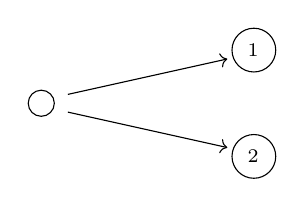
\begin{tikzpicture}[scale=.45]
        \draw [->] (.75,0.25) -- (5.25,1.25);
        \draw [->] (.75,-0.25) -- (5.25,-1.25);
        \node[draw,circle] at (6,1.5) {$\y_1$};
        \node[draw,circle] at (6,-1.5) {$\y_2$};
        \node[draw,circle] at (0,0) {$\x$};
        \node[anchor=south] at (3.5,.75) {};
        \node[anchor=north] at (3.5,-.75) {};
    \end{tikzpicture}
    \caption{General case with arbitrary $f(\{\y_k\}_{k=1}^{K},\x)$}
    \end{figure}
    \begin{definition}[Gel'fand-Pinsker Channel]
    A single user channel with an interference r.v. $W$ \textbf{known to the transmitter}, with p.d.f. $f(Y|X,W)$
    $$C_{GPC}=\sup_{f(X,V|W)}\Inf{V}{Y}-\Inf{V}{W}$$
    where $V$ is an auxiliar r.v.
    \end{definition}
    \pagebreak
    \begin{definition}[Marton's Inner Bound]
    An inner bound $\mathcal{C}_{Marton}\subset \mathcal{C}_{BC}$ based on the GPC.
    $$\bigcup_{f(V_1,V_2,X)} R_1+R_2\leq \Inf{V_1}{Y_1}+\Inf{V_2}{Y_2}-\Inf{V_1}{V_2}$$
    \end{definition}
    \begin{definition}[Cooperative Outter Bound]
    An outer bound to $\mathcal{C}_{BC}\subset\mathcal{C}_{CSB}$ given by assuming receivers can cooperate perfectly. In that case, achieving the cut-set bound $R_1+R_2\leq \Inf{\y_1,\y_2}{\x}$ would be easy using single-user MIMO. 
    \end{definition}
    \begin{remark}
     For arbitrary non-degraded BC channels $\mathcal{C}_{BC}$ is still an open problem. We only focus on \textbf{Gaussian MIMO}.
    \end{remark}
}
\frame[allowframebreaks]{\frametitle{Gaussian MIMO BC Channel}
    \begin{figure}
    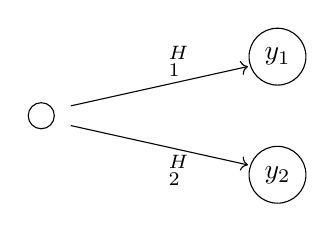
\begin{tikzpicture}[scale=.5]
        \draw [->] (.75,0.25) -- (5.25,1.25);
        \draw [->] (.75,-0.25) -- (5.25,-1.25);
        \node[draw,circle] at (6,1.5) {$y_1$};
        \node[draw,circle] at (6,-1.5) {$y_2$};
        \node[draw,circle] at (0,0) {$\x$};
        \node[anchor=south] at (3.5,.75) {$\h_1^H$};
        \node[anchor=north] at (3.5,-.75) {$\h_2^H$};
    \end{tikzpicture}
    \end{figure}
    \begin{itemize}
     \item $N_t$ transmit antennas\\ \ \\
     \item single-antenna receivers\\ \ \\
     \item \textbf{Not a Degraded BC}\\ \ \\
     \item But $\mathcal{C}_{BC}$ has been solved (Costa)\\ \ \\
     \item The DoF are $\min(K,N_t)$. Moreover, the subset of DoF dedicated to each user $k$ is $\leq1$ because of its single antenna.\\ \ \\
        \begin{definition}[Transmit Signatures]
     We assume that each user is sent a scalar signal $\tilde{x}_k$ with a ``precoding vector'' $\uu_{k}$
     $$\x=\sum_{k}\uu_{k}x_k\textnormal{ where }\Ex{}{|x_k|^2}=P_k$$
    \end{definition}    
    \item Let $\Hb=(\h_1,\dots \h_K)$ and $\U=(\uu_1,\dots \uu_K)$. If $N_t\geq K$ and $\Hb$ is orthogonal we can choose $\uu_k=\h_k/\|\h_k\|^2$ so $$y_k=\Hb^H\U\tilde{\x}+z_k=\tilde{x}_k+z_k$$     
    \item With independent encoding and decoding (supoptimal) linear precoding results in
    $$R_k=\log (1+\gamma_k)\textnormal{ with }\gamma_k=\frac{P_k|\uu_k^H\h_k|^2}{BN_o+\sum_{k'\neq k} P_{k'}|\uu_{k'}^H\h_k|^2}$$
    \item We can design the precoders $\uu_k$'s as filters to maximize the SINRs, weighted sum, etc.\\ \ \\
    \item Maximum SINR with the MMSE receivers \textbf{of the DMAC}\\ \ \\
    \item Linear schemes with superpositon codign are not enough\\ \ \\
    \end{itemize}
}

\frame[allowframebreaks]{\frametitle{MAC -- BC duality (MIMO)}

\begin{columns}[T]
 \begin{column}{6cm}
  $$\y^{BC}=\Hb^H\U\tilde{\x}^{BC}+\z^{BC}$$
  \begin{figure}
%   \resizebox{\columnwidth}{3cm}{
        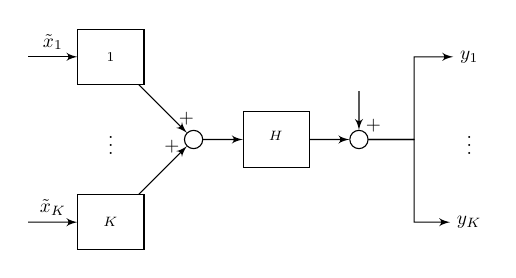
\begin{tikzpicture}[scale=.7, transform shape, auto, node distance=1cm,>=latex']
        \node [input, name=input1] {};
        \node [block, right of=input1, node distance=1.5cm] (prec1) {$\uu_1$};
        \node [below of=prec1, node distance=1.5cm] (prec2) {$\vdots$};
        \node [block, below of=prec2, node distance=1.5cm] (prec3) {$\uu_K$};
        \node [input, left of=prec3, name=input3, node distance=1.5cm] {};
        \draw [draw,->] (input1) -- node {$\tilde{x}_1$} (prec1);
        \draw [draw,->] (input3) -- node {$\tilde{x}_K$} (prec3);
        \node [sum, right of=prec2, node distance=1.5cm] (sum) {};
        \draw [->] (prec1) -- node[anchor=south,pos=0.99] {$+$} (sum);
        \draw [->] (prec3) -- node[anchor=east,pos=0.99] {$+$} (sum);  
        \node [block, right of=sum, node distance=1.5cm] (chan) {$\Hb^H$};    
        \draw [->] (sum) -- (chan);
        \node [sum, right of=chan, node distance=1.5cm] (sz) {};       
        \draw [->] (chan) -- (sz);
        \node [above of=sz, node distance=1cm] (zz) {$\z$};
        \draw [->] (zz) -- node[anchor=west,pos=0.9] {$+$} (sz);
        \coordinate [right of=sz, name=sz2] {};
        \node [right of=sz2, name=output2] {$\vdots$};
        \node [above of=output2, name=output1, node distance=1.5cm] {$y_1$};
        \node [below of=output2, name=output3, node distance=1.5cm] {$y_K$};
        \draw [->] (sz) -- (sz2) |- (output1);
        \draw [->] (sz) -- (sz2) |- (output3);
        \end{tikzpicture}
%         }
    \caption{Gaussian MIMO BC}    
  \end{figure}
 \end{column}
 \begin{column}{6cm}
  $$\y^{DMAC}=\U^H\Hb\tilde{\x}^{DMAC}+\z^{DMAC}$$
  \begin{figure}
        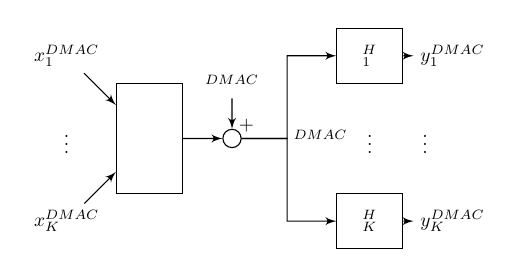
\begin{tikzpicture}[scale=.7, transform shape,auto, node distance=1cm,>=latex']
        \node [name=input1, node distance=1.5cm] {$x^{DMAC}_{1}$};
        \node [below of=input1,name=input2, node distance=1.5cm] {$\vdots$};
        \node [below of=input2,name=input3, node distance=1.5cm] {$x^{DMAC}_{K}$};
        \node [block, minimum height=2cm, right of=input2, node distance=1.5cm] (chan) {$\Hb$};    
        \draw [->] (input1) -- node {} (chan);
        \draw [->] (input3) -- node {} (chan);
        \node [sum, right of=chan, node distance=1.5cm] (sz) {};       
        \draw [->] (chan) -- (sz);
        \node [above of=sz, node distance=1cm] (zz) {$\z^{DMAC}$};
        \draw [->] (zz) -- node[anchor=west,pos=0.9] {$+$} (sz);
        \coordinate [right of=sz, name=sz2];
        \node [right of=sz2, node distance=1.5cm] (prec2) {$\vdots$};
        \node [block, above of=prec2, node distance=1.5cm] (prec1) {$\uu_1^H$};
        \node [block, below of=prec2, node distance=1.5cm] (prec3) {$\uu_K^H$};
        \draw [->] (sz) -- node[anchor=west,pos=0.99] {$\y^{DMAC}$} (sz2) |- (prec1);
        \draw [->] (sz) -- (sz2) |- (prec3); 
        \node [right of=prec2, name=output2] {$\vdots$};
        \node [right of=prec1, name=output1, node distance=1.5cm] {$y_1^{DMAC}$};
        \node [right of=prec3, name=output3, node distance=1.5cm] {$y_K^{DMAC}$};
        \draw [->] (prec1) -- (output1);
        \draw [->] (prec3) -- (output3);
        \end{tikzpicture} 
    \caption{Gaussian MIMO DMAC} 
  \end{figure}
 \end{column}
\end{columns}
\begin{itemize}
 \item The MIMO DMAC employs the signatures as filters $\uu_1^H\dots\uu_K^H$\\ \ \\
 \pagebreak
 \item BC SINRs $\gamma_k=\frac{P_k|\uu_k^H\h_k|^2}{BN_o+\sum_{k'\neq k} P_{k'}|\uu_{k'}^H\h_k|^2}$ \\ \ \\
 \item Denote vector $\ab$ such that $a_k\triangleq\frac{\gamma_k}{(1+\gamma_k)|\h_{k}^H\uu_k|^2}$\\ \ \\
 \item Denote matrix $ \Gb$ such that $G_{k,k'}\triangleq|\uu_{k'}^H\h_{k}|^2$\\ \ \\
 \begin{lemma}
  All DL SINRs are related by the system of linear equations
  $$(\I_K-\Delb_{\ab} \Gb)\vec{P}=N_o\ab \textnormal{ where } \Delb_{\ab}\triangleq\left(\begin{array}{cccc}
                                                                      a_1&0&\dots&0\\
                                                                      0&a_2&\dots&0\\
                                                                      \vdots&\vdots&\ddots&\vdots\\
                                                                      0&0&\dots&a_K\\
                                                                     \end{array}\right)$$
 \end{lemma}
 \pagebreak
 \item DMAC power allocations denoted $Q_k$\\ \ \\
 \item DMAC SINRs $\gamma_k^{DMAC}=\frac{Q_k|\uu_k^H\h_k|^2}{BN_o+\sum_{k'\neq k} Q_{k'}|\uu_k^H\h_{k'}|^2}$\\ \ \\
 \begin{itemize}
    \item DMAC ``all the $\h$'s to $\uu_k$'' vs BC ``all the $\uu$'s to $\h_k$''\\ \ \\
 \end{itemize}
 \item Denote vector $\bb$ such that $b_k\triangleq\frac{\gamma_k^{DMAC}}{(1+\gamma_k^{DMAC})|\h_{k}^H\uu_k|^2}$
 \begin{lemma}
  All UL SINRs are related by the system of linear equations
  $$(\I_K-\Delb_{\bb} \Gb^T)\vec{Q}=N_o\bb$$
 \end{lemma}
 \pagebreak
 \item We can solve for $\vec{P}$ and $\vec{Q}$ respectively ($\Delb_{\bb}^{-1}\bb=\one_K$)
 $$\vec{P}=N_o(\Delb_{\ab}^{-1}- \Gb)^{-1}\one_{K}$$
 $$\vec{Q}=N_o(\Delb_{\bb}^{-1}- \Gb^T)^{-1}\one_{K}$$
 
 \begin{theorem} The same SINRs can be achieved with the same \textbf{sum of} power
 \begin{equation}
 \begin{split}
 \gamma_k=\gamma_k^{DMAC} \Rightarrow \ab=\bb \Rightarrow
  \sum_{k=1}^{K}P_k&=N_o\one_{K}^T(\Delb_{\ab}^{-1}- \Gb)^{-1}\one_{K}\\
    &=N_o\one_{K}^T(\Delb_{\bb}^{-1}- \Gb^T)^{-1}\one_{K}\\
    &=\sum_{k=1}^{K}Q_k
  \end{split}
 \end{equation}
 \end{theorem}
 \pagebreak
    \item Assuming $\vec{Q}$ fixed we can find optimal $\uu_k$ \textbf{in DMAC} (MMSE)\\ \ \\
    \item Assuming $\uu_k$ fixed we can choose $\vec{Q}$ \textbf{in DMAC} (dual problem)\\ \ \\
    \item We can use iterative updates of both (marginal subproblems)
    $$\vec{Q}^{(n)}\to\{\uu_k^{(n)}\}_{k=1}^{K}\to \vec{Q}^{(n+1)}$$\\ \ \\
    \item Finally we compute $\bb$ using $\vec{Q}$, and $\vec{P}$ using $\ab=\bb$\\ \ \\
\end{itemize}
}


\frame[allowframebreaks]{\frametitle{Non-linear BC Transmitter Schemes}
    \begin{itemize}
     \item To achieve Gaussian BC $\mathcal{C}$ we need to cancel interference\\ \ \\
     \item In SISO, strongest receiver can decode everything (recursive) \\ \ \\
     \item In MIMO there is no ``receiver order''\\ \ \\
     \item \textbf{Only the BS} knows all transmitted signals: Is there some method equivalent to SIC at the transmitter?\\ \ \\
    \end{itemize}
}

\frame[allowframebreaks]{\frametitle{Na\"ive pre-canceller}
    \begin{itemize}
     \item Suppose an AWGN channel with known interference
     $$y=x+w+z$$
    \vspace{-.3in}
     \begin{itemize}
        \item $x$ is the transmitted signal
        \item $w$ is \textbf{known} to the transmitter
        \item $z$ is the noise\\ \ \\
     \end{itemize}
     
     \item If $\Ex{}{|w|^2}<P$ we could send $x=v-w$, where $v$ is the desired signal
     \item Then the rate would be
     $R_{\textnormal{na\"ive}}=\log_2\left(1+\frac{P-\Ex{}{|w|^2}}{BN_o}\right)$\\ \ \\
     \item We could only cancel \textbf{partially} $x=v-\alpha w$ with $\alpha\in[0,1]$
     $$R_{\alpha-\textnormal{na\"ive}}=\log_2\left(1+\frac{P-\alpha\Ex{}{|w|^2}}{(1-\alpha)\Ex{}{|w|^2}+BN_o}\right)$$\\ \ \\
    \end{itemize}
}


\frame[allowframebreaks]{\frametitle{Dirty Paper Coding}
     \begin{Theorem}[Costa'83]
      Using Dirty Paper Coding (DPC) a transmitter that knows the interference can achieve rate
     $$R_{DPC}=\log_2\left(1+\frac{P}{BN_o}\right)$$
     \end{Theorem}
     \begin{columns}
      \begin{column}{5.5cm}
      \begin{itemize}
       \item \textcolor{ARust}{Same rate as AWGN case!}\\ \ \\
        \item An application of the Gel'fand and Pinsker Channel\\ \ \\
      \end{itemize}
      \end{column}
      \begin{column}{4cm}
      \begin{figure}
      \centering
       \begin{tikzpicture}[scale=.55]
       \begin{axis}[
            axis lines = left,
            xlabel = $\alpha$,
            ylabel = {$R$},
            ymax=4,
            legend style={at={(.95,.53)}}
        ]
        \addplot [thick,
            domain=0:1, 
            samples=100, 
            color=ARust,
        ]
        {ln(1+10)/ln(2)};
        \addlegendentry{$C_{AWGN}$ with $P/BN_o=10$dB}
        \addplot [dashed,thick,
            domain=0:1, 
            samples=100, 
            color=VCobalt,
        ]
        {ln(1+(10-x)/(1+(1-x))/ln(2)};
        \addlegendentry{$R_{\alpha-\textnormal{na\"ive}}|w|^2=P/10$}
        \addplot [dotted,thick,
            domain=0:1, 
            samples=100, 
            color=KYJade,
        ]
        {ln(1+(10-10*x)/(1+10*(1-x))/ln(2)};
        \addlegendentry{$R_{\alpha-\textnormal{na\"ive}}|w|^2=P$}
        \end{axis}
        \end{tikzpicture} 
        \end{figure}
      \end{column}
     \end{columns}     
     \pagebreak
     
    \begin{itemize}
     \item Let $\textcolor{KYJade}{r}=\textcolor{VCobalt}{x}+\textcolor{ARust}{w}$ denote the \textit{noiseless signal+interference}\\ \ \\
     \item The na\"ive scheme spends power going \textit{against} interference
 \begin{figure}
        \begin{tikzpicture}[scale=.8]
        \draw[dotted,gray,<->] (-2,0) -- (2,0);
        \fill[KYJade] (-1,0) circle (.1);
        \node[regular polygon,regular polygon sides=3, inner sep=1.3,minimum size=.1, fill=KYJade] at (1,0) {};
        \draw[black] (0,.1) -- (0,-.1);
        \node[anchor=north] at (0,0) {$0$};
        \node[color=KYJade,anchor=north] at (-1,0) {$r_{_{-1}}$};
        \node[color=KYJade,anchor=north] at (1,0) {$r_{_{+1}}$};
%         \draw (1.4,-0.1) rectangle (1.6,0.1);
        \fill[ARust] (1.4,-0.1) rectangle (1.6,0.1);
        \node[color=ARust,anchor=north] at (1.5,0) {$w$};
        \draw [color=VCobalt,->] (1.5,.1) to [out=150,in=30] node[anchor=south] {$x_{_{-1}}$} (-1,.1);
        \draw [color=VCobalt,->] (1.5,.1) to [out=135,in=45] node[anchor=east] {$x_{_{+1}}$} (1,.1);
        \end{tikzpicture} 
%     \caption{BPSK $r$ in the na\"ive scheme} 
  \end{figure}
     \item Define \textit{lattice} $\Lambda_{BPSK}=\bigcup_{d=-\infty}^{\infty}\{\textnormal{BPSK}-4d\}$
     \begin{itemize}
        \item Infinite copies of \textnormal{BPSK} constellation along real line.
     \end{itemize}
     
 \begin{figure}
        \begin{tikzpicture}[scale=.7]
        \draw[dotted,gray,<->] (-5.5,0) -- (5.5,0);           
            \foreach \x in {-1,0,...,1} { 
            \fill[KYJade] (4*\x-1,0) circle (.1);
%             \fill[KYJade] (4*\x+1,0) circle (.1);
            \node[regular polygon,regular polygon sides=3, inner sep=1.3,minimum size=.1, fill=KYJade] at (4*\x+1,0) {};
            \node[color=KYJade,anchor=north] at (4*\x-1,0) {$r_{_{-1}}$};
            \node[color=KYJade,anchor=north] at (4*\x+1,0) {$r_{_{+1}}$};
        }
        \draw[black] (0,.1) -- (0,-.1);
        \node[anchor=north] at (0,0) {$0$};
        \fill[ARust] (1.4,-0.1) rectangle (1.6,0.1);
        \node[color=ARust,anchor=north] at (1.5,0) {$w$};
        \draw [color=VCobalt,->] (1.5,.1) to [out=45,in=135] node[anchor=south] {$x_{_{-1}}$} (3 ,.1);
        \draw [color=VCobalt,->] (1.5,.1) to [out=135,in=45] node[anchor=south] {$x_{_{+1}}$} (1,.1);
        \end{tikzpicture} 
    \caption{Tomlinson-Harashima BPSK scheme} 
  \end{figure}
     \pagebreak
     \item DPC chooses $x$ \textit{in the same direction of $w$, not against it}
         $$\forall w\in \mathbb{R}\; \Ex{}{|x|^2}=\Ex{}{|r_{_{\textnormal{DPC}}}-w|^2}=1=\Ex{}{BPSK}$$\\ \ \\
     \item Nested lattice Decoding
        \begin{itemize}
            \item $\Lambda_{BPSK}$ is a union of sublattices 
            $$\textcolor{ARust}{\Lambda_{+1}=\bigcup_{d=-\infty}^{\infty}\{1-4d\}}\textnormal{ and }\textcolor{VCobalt}{\Lambda_{-1}=\bigcup_{d=-\infty}^{\infty}\{-1-4d\}}$$
            \item Identify noiseless symbol $\displaystyle\hat{r}=\arg\min_{\Lambda_{const}=\bigcup \Lambda_{n}} \|y-r\|^2$\\ \ \\
            \item Identify the sublattice $\hat{n}=\textnormal{find}\{n : \hat{r}\in \Lambda_{n}\} $
     \\ \ \\
        \end{itemize}
 \begin{figure}
        \begin{tikzpicture}[scale=.9]
        \draw[dotted,gray,<->] (-5.5,0) -- (5.5,0);           
            \foreach \x in {-1,0,...,1} { 
            \fill[VCobalt] (4*\x-1,0) circle (.1);
            \node[regular polygon,regular polygon sides=3, inner sep=1.3,minimum size=.1, fill=ARust] at (4*\x+1,0) {};
            \node[color=VCobalt,anchor=north] at (4*\x-1,0) {$v_{_{-1}}$};
            \node[color=ARust,anchor=north] at (4*\x+1,0) {$v_{_{+1}}$};
        }
        \end{tikzpicture} 
  \end{figure}
     \pagebreak
        \begin{figure}
        \begin{tikzpicture}[scale=.5]
        \tikzset{mark options={mark size=3}}
            \begin{axis}[
            axis x line=center,
            axis y line=center,
            xmin=-1,xmax=1,
            ymin=-1, ymax=1,
            xtick={-1,...,1},
            xticklabels={,,},
            ytick={-1,...,1},
            yticklabels={,,},
            scatter/classes={%
                a={mark=*,color=VCobalt},
                b={mark=triangle*,color=ARust},
                c={mark=square*,color=KYJade},
                d={mark=diamond*,color=TAMustard}}]

        \addplot[scatter,only marks,%
            scatter src=explicit symbolic]%
            table[meta=label]{
                x         y       label
                0.6424    0.5605  a
                -0.9692   -0.8377 a
                -0.9140   0.8588  a
                -0.6620   0.5514  a
                0.2982    -0.0264 a
                0.4634    -0.1283 a
                0.2955    -0.1064 a
                -0.0982   -0.3873 a
                0.0940    0.0170  b
                -0.4074   0.0215  b
                0.4894    0.6353  b
                -0.6221   0.5897  b
                0.3736    0.2886  b
                -0.6330   -0.2428 b
                -0.2630   0.6232  b
                0.2512    0.0657  b
                -0.2985   -0.3778 c
                0.8780    0.8468  c
                0.7519   -0.1396  c
                0.1003   -0.6304  c
                0.2450    0.8098  c
                0.1741    0.9595  c
                -0.5845   -0.1223 c
                -0.3975   -0.7778 c
                -0.0582   -0.4839 d
                -0.5390   -0.1826 d
                0.6886    0.1898  d
                -0.6105   -0.4756 d
                -0.5482    0.2057 d
                -0.6586    0.4224 d
                -0.5447   -0.5565 d
                -0.1286   -0.7652 d
        };
        \addplot[scatter,only marks,%
            scatter src=explicit symbolic,%
            mark=pentagon*,color=black]%
            coordinates {(.2,.6)
        };
        \node (destination) at (axis cs:0.4894,0.6353){};
        \draw [color=black,->] (axis cs:.2,.6){} to [out=-45,in=-135] node[anchor=north] {$x_{_{1}}$} (destination);
        \end{axis}
        \end{tikzpicture}    
        \end{figure}        
     \item General DPC proof by Costa 
     \begin{itemize}
        \item $N_Q$ random quantizers $\mathscr{Q}_{n}()$ in $\mathbb{C}^{N}$
        \item \textcolor{ARust}{Encoder $\x_{n}=\mathscr{Q}_{n}(\w)-\alpha\w$}, $\Ex{}{\|\x\|^2}\leq P$ $\Rightarrow$ $2^{\Inf{\rr}{\w}}$ points
        \item Union quantizer $\displaystyle \mathscr{Q}_{tot}()=\bigcup_{n=1}^{2^R} \mathscr{Q}_{n}()$
        \item Reliable detection against noise $\hat{\rr}=\mathscr{Q}_{tot}(\y)$ with $2^{\Inf{\y}{\rr}}$ points
        \begin{equation}
         \begin{split}
            R&=\log_2 N_Q=\log_2\frac{2^{\Inf{\y}{\rr}}}{2^{\Inf{\rr}{\w}}}=\Inf{\y}{\rr}-\Inf{\rr}{\w}
         \end{split}
        \end{equation}
     \end{itemize}
     \pagebreak
     \item Distortion Compensation $\x_{n}=\mathscr{Q}_{n}(\w)-\underset{\textnormal{DC}}{\underbrace{\alpha\w}}$
     \begin{itemize}
        \item Costa simplifies '$\displaystyle \max_{f(\rr,\x)}$ of GPC' to linear $\rr=\mathscr{Q}_{n}(\w)+(1-\alpha)\w$\\ \ \\
        \item Optimal $\alpha^*=\frac{P}{P+\sigma_z^2}$ (Not full cancelling!)\\ \ \\
     \end{itemize}
     \item Quantization Index Modulation (QIM) [Chen \& Wornell'98]
    \end{itemize}
    \begin{columns}[T]
      \begin{column}{6cm}
       \begin{figure}
        \centering
        \includegraphics[width=.6\columnwidth]{lattice}
        \end{figure}
      \end{column}
      \begin{column}{6cm}
       \begin{itemize}
        \item a.k.a. Dither Modulation (DM)    \\ \ \\
        \item Regular Nested Lattices in $\mathbb{C}^{N}$
        $$\Lambda_n=\Lambda_0+\mathbf{d}_n \forall n\in\{0,2^{R}\}$$
        \item DC in practice too
     \end{itemize}
      \end{column}
     \end{columns}
}

\frame[allowframebreaks]{\frametitle{\small Achieving Gaussian MIMO BC Capacity (DPC+Duality)}
    \begin{itemize}
     \item For decoding order $\pi(1),\pi(2),\dots,\pi(K)=1\dots K$\\ \ \\
     \item Write the signal received by user $k$ as
     $$y_k=\h_k^H\uu_k\tilde{x}_k+\underset{\textnormal{DPC}}{\underbrace{\sum_{k'=1}^{k-1}\h_k^H\uu_{k'}\tilde{x}_{k'}}}+\underset{\textnormal{DMAC equations}}{\underbrace{\sum_{k'=k+1}^{K}\h_k^H\uu_k\tilde{x}_k}}$$
        \begin{itemize}
            \item $\gamma_k=\frac{P_k|\uu_k^H\h_k|^2}{BN_o+\sum_{\textcolor{ARust}{k'> k}} P_{k'}|\uu_{k'}^H\h_k|^2}$
            \item $\gamma_k^{DMAC}=\frac{P_k|\uu_k^H\h_k|^2}{BN_o+\sum_{\textcolor{ARust}{k'< k}} P_{k'}|\uu_k^H\h_{k'}|^2}$
            \item $\{\uu_k\}_{k=1}^{K}\rightleftharpoons \vec{Q}\to \ab=\bb\to\vec{P}$
        \end{itemize}
%      \pagebreak
%         \item Receive Beamforming (MMSE) + SIC receiver achieves $\mathcal{C}_{MAC}$\\ \ \\
%         \item Transmit Beamforming + DPC transmitter achieves $\mathcal{C}_{BC}$\\ \ \\
%         \item For MIMO, $\mathcal{C}_{BC}$ cannot be achieved with superposition coding\\ \ \\
    \end{itemize}

}
% \frame[allowframebreaks]{\frametitle{}
% 
% Consider the DMAC of a MIMO BC using linear filters $\uu_i$ and DPC. The decoding order is 1, 2, 3 ...
% \begin{itemize}
%  \item The BC SINR is \(\gamma_i=\) \\ \ \\
%  \item The DMAC SINR is \(\gamma_i^{DMAC}=\) \\ \ \\
% \end{itemize}
% 
%     \(\frac{|\mathbf{u}_i^H\mathbf{h}_i|P_i}{\sigma^2_z+\sum_{k'\neq i}|\mathbf{u}_{k'}^H\mathbf{h}_i|P_{k'}}\)
%     
%     \(\frac{|\mathbf{u}_i^H\mathbf{h}_i|P_i}{\sigma^2_z+\sum_{k'\neq i}|\mathbf{u}_i^H\mathbf{h}_{k'}|P_{k'}}\)
%     
%     \(\frac{|\mathbf{u}_i^H\mathbf{h}_i|P_i}{\sigma^2_z+\sum_{j= i+1}^{N}|\mathbf{u}_{k'}^H\mathbf{h}_i|P_{k'}}\)
%     
%     \(\frac{|\mathbf{u}_i^H\mathbf{h}_i|P_i}{\sigma^2_z+\sum_{j= 1}^{i-1}|\mathbf{u}_i^H\mathbf{h}_{k'}|P_{k'}}\)
%     }
    
\end{document}


